\documentclass[conference]{IEEEtran}
\IEEEoverridecommandlockouts
\usepackage{cite}
\usepackage{amsmath,amssymb,amsfonts}
\usepackage{graphicx}
\usepackage{textcomp}
\usepackage{xcolor}
\usepackage{booktabs}
\usepackage{subcaption}
\usepackage{url}
\graphicspath{{../results/figures/}}
% AUTO-GENERATED by scripts/make_paper_numbers.py -- do not edit by hand.

\newcommand{\accTestOne}{84.4}
\newcommand{\foneTestOne}{84.4}
\newcommand{\accValOne}{78.8}
\newcommand{\accCanOne}{64.0}
\newcommand{\foneCanOne}{63.6}
\newcommand{\gapOne}{20.4}
\newcommand{\eceTestOne}{0.161}
\newcommand{\eceCanOne}{0.145}
\newcommand{\trainTimeOne}{4.0}
\newcommand{\epochSecOne}{20}
\newcommand{\epochsOne}{12}
\newcommand{\bestEpochOne}{12}
\newcommand{\trainAccOne}{81.3}
\newcommand{\paramsOne}{11.19}
\newcommand{\macsOne}{1.82}
\newcommand{\latGpuOne}{3.4}
\newcommand{\latCpuOne}{16.8}
\newcommand{\fpsGpuOne}{295}
\newcommand{\accTestTwo}{84.1}
\newcommand{\foneTestTwo}{84.0}
\newcommand{\accValTwo}{78.6}
\newcommand{\accCanTwo}{64.3}
\newcommand{\foneCanTwo}{63.8}
\newcommand{\gapTwo}{19.8}
\newcommand{\eceTestTwo}{0.157}
\newcommand{\eceCanTwo}{0.142}
\newcommand{\trainTimeTwo}{5.6}
\newcommand{\epochSecTwo}{28}
\newcommand{\epochsTwo}{12}
\newcommand{\bestEpochTwo}{10}
\newcommand{\trainAccTwo}{77.4}
\newcommand{\paramsTwo}{11.19}
\newcommand{\macsTwo}{1.82}
\newcommand{\latGpuTwo}{3.2}
\newcommand{\latCpuTwo}{15.5}
\newcommand{\fpsGpuTwo}{312}
\newcommand{\accTestThree}{89.7}
\newcommand{\foneTestThree}{89.8}
\newcommand{\accValThree}{85.0}
\newcommand{\accCanThree}{64.0}
\newcommand{\foneCanThree}{63.7}
\newcommand{\gapThree}{25.7}
\newcommand{\eceTestThree}{0.118}
\newcommand{\eceCanThree}{0.079}
\newcommand{\trainTimeThree}{3.8}
\newcommand{\epochSecThree}{19}
\newcommand{\epochsThree}{12}
\newcommand{\bestEpochThree}{8}
\newcommand{\trainAccThree}{99.5}
\newcommand{\paramsThree}{11.19}
\newcommand{\macsThree}{1.82}
\newcommand{\latGpuThree}{3.8}
\newcommand{\latCpuThree}{17.1}
\newcommand{\fpsGpuThree}{264}
\newcommand{\accTestFour}{90.5}
\newcommand{\foneTestFour}{90.5}
\newcommand{\accValFour}{85.4}
\newcommand{\accCanFour}{66.0}
\newcommand{\foneCanFour}{65.8}
\newcommand{\gapFour}{24.5}
\newcommand{\eceTestFour}{0.124}
\newcommand{\eceCanFour}{0.077}
\newcommand{\trainTimeFour}{5.9}
\newcommand{\epochSecFour}{29}
\newcommand{\epochsFour}{12}
\newcommand{\bestEpochFour}{11}
\newcommand{\trainAccFour}{98.0}
\newcommand{\paramsFour}{11.19}
\newcommand{\macsFour}{1.82}
\newcommand{\latGpuFour}{3.7}
\newcommand{\latCpuFour}{17.0}
\newcommand{\fpsGpuFour}{270}
\newcommand{\accTestFive}{81.9}
\newcommand{\foneTestFive}{81.9}
\newcommand{\accValFive}{75.6}
\newcommand{\accCanFive}{57.2}
\newcommand{\foneCanFive}{57.3}
\newcommand{\gapFive}{24.7}
\newcommand{\eceTestFive}{0.146}
\newcommand{\eceCanFive}{0.150}
\newcommand{\trainTimeFive}{4.9}
\newcommand{\epochSecFive}{24}
\newcommand{\epochsFive}{12}
\newcommand{\bestEpochFive}{11}
\newcommand{\trainAccFive}{74.5}
\newcommand{\paramsFive}{1.54}
\newcommand{\macsFive}{0.06}
\newcommand{\latGpuFive}{5.8}
\newcommand{\latCpuFive}{9.0}
\newcommand{\fpsGpuFive}{173}
\newcommand{\accTestSix}{66.0}
\newcommand{\foneTestSix}{65.7}
\newcommand{\accValSix}{59.1}
\newcommand{\accCanSix}{35.6}
\newcommand{\foneCanSix}{35.0}
\newcommand{\gapSix}{30.4}
\newcommand{\eceTestSix}{0.095}
\newcommand{\eceCanSix}{0.085}
\newcommand{\trainTimeSix}{7.4}
\newcommand{\epochSecSix}{37}
\newcommand{\epochsSix}{12}
\newcommand{\bestEpochSix}{11}
\newcommand{\trainAccSix}{66.8}
\newcommand{\paramsSix}{11.19}
\newcommand{\macsSix}{1.82}
\newcommand{\latGpuSix}{4.4}
\newcommand{\latCpuSix}{16.2}
\newcommand{\fpsGpuSix}{230}
\newcommand{\accTestSeven}{91.7}
\newcommand{\foneTestSeven}{91.6}
\newcommand{\accValSeven}{86.7}
\newcommand{\accCanSeven}{71.6}
\newcommand{\foneCanSeven}{71.6}
\newcommand{\gapSeven}{20.1}
\newcommand{\eceTestSeven}{0.113}
\newcommand{\eceCanSeven}{0.089}
\newcommand{\trainTimeSeven}{63.1}
\newcommand{\epochSecSeven}{316}
\newcommand{\epochsSeven}{12}
\newcommand{\bestEpochSeven}{12}
\newcommand{\trainAccSeven}{90.6}
\newcommand{\accTestEight}{91.8}
\newcommand{\foneTestEight}{91.8}
\newcommand{\accValEight}{87.2}
\newcommand{\accCanEight}{70.9}
\newcommand{\foneCanEight}{70.8}
\newcommand{\gapEight}{20.9}
\newcommand{\eceTestEight}{0.115}
\newcommand{\eceCanEight}{0.083}
\newcommand{\trainTimeEight}{53.0}
\newcommand{\epochSecEight}{265}
\newcommand{\epochsEight}{12}
\newcommand{\bestEpochEight}{11}
\newcommand{\trainAccEight}{90.6}
\newcommand{\accTestNine}{83.4}
\newcommand{\foneTestNine}{83.4}
\newcommand{\accValNine}{78.9}
\newcommand{\accCanNine}{60.6}
\newcommand{\foneCanNine}{60.0}
\newcommand{\gapNine}{22.8}
\newcommand{\eceTestNine}{0.154}
\newcommand{\eceCanNine}{0.188}
\newcommand{\trainTimeNine}{44.2}
\newcommand{\epochSecNine}{221}
\newcommand{\epochsNine}{12}
\newcommand{\bestEpochNine}{9}
\newcommand{\trainAccNine}{67.2}
\newcommand{\accTestTen}{83.0}
\newcommand{\foneTestTen}{83.0}
\newcommand{\accValTen}{78.5}
\newcommand{\accCanTen}{61.8}
\newcommand{\foneCanTen}{61.4}
\newcommand{\gapTen}{21.2}
\newcommand{\eceTestTen}{0.174}
\newcommand{\eceCanTen}{0.227}
\newcommand{\trainTimeTen}{51.4}
\newcommand{\epochSecTen}{257}
\newcommand{\epochsTen}{12}
\newcommand{\bestEpochTen}{9}
\newcommand{\trainAccTen}{66.8}
\newcommand{\accTestEleven}{83.2}
\newcommand{\foneTestEleven}{83.2}
\newcommand{\accValEleven}{78.8}
\newcommand{\accCanEleven}{61.1}
\newcommand{\foneCanEleven}{60.7}
\newcommand{\gapEleven}{22.1}
\newcommand{\eceTestEleven}{0.162}
\newcommand{\eceCanEleven}{0.204}
\newcommand{\trainTimeEleven}{49.3}
\newcommand{\epochSecEleven}{246}
\newcommand{\epochsEleven}{12}
\newcommand{\bestEpochEleven}{10}
\newcommand{\trainAccEleven}{66.9}
\newcommand{\accTestTwelve}{91.0}
\newcommand{\foneTestTwelve}{90.9}
\newcommand{\accValTwelve}{86.4}
\newcommand{\accCanTwelve}{71.4}
\newcommand{\foneCanTwelve}{71.4}
\newcommand{\gapTwelve}{19.6}
\newcommand{\eceTestTwelve}{0.107}
\newcommand{\eceCanTwelve}{0.082}
\newcommand{\trainTimeTwelve}{115.9}
\newcommand{\epochSecTwelve}{290}
\newcommand{\epochsTwelve}{24}
\newcommand{\bestEpochTwelve}{18}
\newcommand{\trainAccTwelve}{95.5}
\newcommand{\accTestFourSeed}{90.1}
\newcommand{\foneTestFourSeed}{90.1}
\newcommand{\accValFourSeed}{84.5}
\newcommand{\accCanFourSeed}{66.5}
\newcommand{\foneCanFourSeed}{66.4}
\newcommand{\gapFourSeed}{23.6}
\newcommand{\eceTestFourSeed}{0.119}
\newcommand{\eceCanFourSeed}{0.082}
\newcommand{\trainTimeFourSeed}{9.8}
\newcommand{\epochSecFourSeed}{49}
\newcommand{\epochsFourSeed}{12}
\newcommand{\bestEpochFourSeed}{10}
\newcommand{\trainAccFourSeed}{97.9}

\newcommand{\gainAugFrozen}{-0.3}
\newcommand{\gainAugFinetune}{+0.8}
\newcommand{\gainFinetuneNoaug}{+5.3}
\newcommand{\gainFinetuneAug}{+6.4}
\newcommand{\gainMobile}{-8.6}
\newcommand{\gainCanFinetuneNoaug}{+0.0}
\newcommand{\gainCanFinetuneAug}{+1.7}
\newcommand{\gainCanAugFrozen}{+0.3}
\newcommand{\gainCanAugFinetune}{+2.0}
\newcommand{\gainExternal}{+1.2}
\newcommand{\gainCanExternal}{+5.6}
\newcommand{\gainTarget}{1.2}
\newcommand{\leakTest}{+0.1}
\newcommand{\leakCan}{-0.7}
\newcommand{\gainDataMobile}{+1.5}
\newcommand{\gainCanDataMobile}{+3.4}
\newcommand{\kdOneTest}{-0.4}
\newcommand{\kdOneCan}{+1.2}
\newcommand{\kdTwoTest}{-0.2}
\newcommand{\kdTwoCan}{+0.5}
\newcommand{\kdOneVal}{-0.4}
\newcommand{\kdTwoVal}{-0.2}
\newcommand{\gainMobileCost}{8.6}
\newcommand{\speedCpuFive}{47}
\newcommand{\slowGpuFive}{56}
\newcommand{\gainScratch}{-24.5}
\newcommand{\gainCanScratch}{-30.4}
\newcommand{\scratchDrop}{24.5}
\newcommand{\scratchDropCan}{30.4}
\newcommand{\tempOne}{0.66}
\newcommand{\eceTestCalOne}{0.034}
\newcommand{\eceCanCalOne}{0.050}
\newcommand{\tempTwo}{0.68}
\newcommand{\eceTestCalTwo}{0.038}
\newcommand{\eceCanCalTwo}{0.034}
\newcommand{\tempThree}{0.72}
\newcommand{\eceTestCalThree}{0.023}
\newcommand{\eceCanCalThree}{0.055}
\newcommand{\tempFour}{0.70}
\newcommand{\eceTestCalFour}{0.022}
\newcommand{\eceCanCalFour}{0.061}
\newcommand{\tempFive}{0.70}
\newcommand{\eceTestCalFive}{0.033}
\newcommand{\eceCanCalFive}{0.021}
\newcommand{\tempSix}{0.84}
\newcommand{\eceTestCalSix}{0.030}
\newcommand{\eceCanCalSix}{0.134}
\newcommand{\tempSeven}{0.74}
\newcommand{\eceTestCalSeven}{0.028}
\newcommand{\eceCanCalSeven}{0.041}
\newcommand{\tempEight}{0.72}
\newcommand{\eceTestCalEight}{0.020}
\newcommand{\eceCanCalEight}{0.042}
\newcommand{\tempNine}{0.65}
\newcommand{\eceTestCalNine}{0.022}
\newcommand{\eceCanCalNine}{0.039}
\newcommand{\tempTen}{0.61}
\newcommand{\eceTestCalTen}{0.017}
\newcommand{\eceCanCalTen}{0.039}
\newcommand{\tempEleven}{0.63}
\newcommand{\eceTestCalEleven}{0.016}
\newcommand{\eceCanCalEleven}{0.038}
\newcommand{\ttaHflipTestFour}{91.2}
\newcommand{\ttaFiveTestFour}{91.2}
\newcommand{\ttaScalesTestFour}{90.8}
\newcommand{\ttaHflipCanFour}{67.9}
\newcommand{\ttaFiveCanFour}{66.2}
\newcommand{\ttaScalesCanFour}{66.0}
\newcommand{\ttaHflipResampleFour}{65.8}
\newcommand{\ttaFiveResampleFour}{67.5}
\newcommand{\ttaScalesResampleFour}{63.0}
\newcommand{\ttaHflipTestSeven}{92.5}
\newcommand{\ttaFiveTestSeven}{92.9}
\newcommand{\ttaScalesTestSeven}{92.1}
\newcommand{\ttaHflipCanSeven}{72.6}
\newcommand{\ttaFiveCanSeven}{71.4}
\newcommand{\ttaScalesCanSeven}{69.4}
\newcommand{\ttaHflipResampleSeven}{69.2}
\newcommand{\ttaFiveResampleSeven}{69.8}
\newcommand{\ttaScalesResampleSeven}{66.0}
\newcommand{\redrawCanFour}{63.6}
\newcommand{\redrawCanSeven}{67.6}
\newcommand{\redrawGapSeven}{4.0}


\begin{document}

\title{Chinese Canteen Dish Recognition with Calorie-Range Estimation: Pre-Training Scale, Open-Set Gating and Cross-Domain Evaluation}

\author{\IEEEauthorblockN{Student Name}
\IEEEauthorblockA{School of Computer Science and Technology \\
University, City, China \\
student@example.edu}
}

\maketitle

\begin{abstract}
Photographing a canteen tray and receiving a rough energy range is a practical
way to raise nutritional awareness among students, but a canteen serves a menu
that no public dataset contains: the dishes are Chinese, the photographs are
hand-held, and a twenty-way classifier always answers, even when the plate holds
something it has never seen. This paper reports a controlled study of that
setting. We start from CNFOOD-241, a 241-class Chinese dish dataset, and
pre-train a ResNet-18 on \cnPreTrainN{} images before fitting a 21-way canteen
head (twenty dishes plus a catch-all bucket) on \cnTrainN{} images. Pre-training
raises test accuracy from \cnNoPreTest\% to \cnTest\% with the same recipe, and a
six-view test-time fusion adds \cnFuseGain{} points on top, reaching
\cnFuseTop\% top-1 and \cnFuseTopFive\% top-5 on \cnTestN{} held-out photographs.
The twenty dish rows of the confusion matrix reach \cnDishAcc\%, but the
catch-all bucket is only \cnOtherRecall\% recalled, which is why we treat
open-set behaviour as a first-class result rather than a footnote: a domain
probe on pooled features plus a Chinese-dish veto decides whether the system
names a dish at all. On five evaluation sets the gate keeps \gateIn\% of canteen
photographs, \gateVal\% of the validation split, but admits only \gateOutCn\% of
fifteen unseen Chinese dishes, \gateOutOther\% of non-food scenes and
\gateReal\% of a real-photograph probe, at the cost of \gateInCost{} points of
coverage on the supported set. On \webN{} web images of the twenty dishes,
screened for near-duplicates against the training data, the system is
\webTop\% top-1 accurate and accepts \webAccept\%. Three follow-up experiments
are negative: stronger photometric augmentation, class-balanced and focal losses
move accuracy by less than the seed spread, which locates the remaining error in
intra-class variation and in the boundary of the catch-all class rather than in
the optimisation.
\end{abstract}

\begin{IEEEkeywords}
Chinese food recognition, canteen tray, transfer learning, pre-training scale,
open-set recognition, calibration, calorie estimation
\end{IEEEkeywords}

\section{Introduction}
\IEEEPARstart{C}{anteen} meals are the main source of daily energy for most
Chinese university students, yet the energy content of a dish is rarely visible
at the point of choice. A system that takes a single photograph of a tray and
returns the three most likely dishes together with a rough energy interval would
make calorie awareness immediate, requires no wearable sensor and no manual
logging, and can run on a commodity laptop or an edge device.

Building such a system is not simply an image-classification exercise, and the
difficulty is not the one a Western benchmark suggests. First, the menu is
Chinese: the dishes a canteen serves---mapo tofu, braised pork, stir-fried potato
shreds, steamed egg---are almost absent from Food-101, so a model trained on the
usual benchmark answers a question nobody asked. Second, the photographs are
taken with hand-held phones under mixed artificial light, at oblique angles, with
cluttered trays, partially eaten portions and steam, and a classifier trained on
curated studio photographs degrades sharply under this shift
\cite{hendrycks2019robustness}. Third, and most awkwardly for a deployed system,
a softmax classifier always returns a class: when the tray holds a dish outside
the menu, or no dish at all, the model still produces a confident answer. Since
the number of dishes a canteen serves is large and the frequency distribution is
skewed, the useful question is not only \emph{which} dish but \emph{whether to
answer at all}.

This paper therefore studies three things that a course-scale project can
actually control. We ask how much Chinese pre-training is worth by fitting the
same canteen head twice, once from ImageNet weights and once from a backbone
pre-trained on 241 Chinese dish classes. We ask how much test-time fusion of
several framings is worth, since a tray photograph has no canonical crop. And we
ask how a deployed system should decline to answer, which we treat as a
measurable quantity on five evaluation sets rather than as a threshold chosen by
eye.

Our contributions are:
\begin{itemize}
\item a 21-way Chinese canteen protocol built on CNFOOD-241 \cite{cnfood241}
with a leak-free split, a 241-class pre-training stage, and a catch-all bucket
that makes "some other dish" an explicit class instead of a silent error;
\item a controlled measurement of pre-training scale: the identical recipe and
head move from \cnNoPreTest\% to \cnTest\% test accuracy when the backbone is
pre-trained on Chinese dishes (\cnGainPretrain{} points), which is larger than
any adaptation-policy change we could obtain on the Western benchmark;
\item a six-view test-time fusion whose gain (\cnFuseGain{} points) is measured
against the single-view protocol used for model selection, and a per-class error
analysis that locates the residual error in intra-class variation
(sweet-and-sour ribs versus sweet-and-sour pork, twice-cooked pork versus
braised pork) rather than in class imbalance;
\item an open-set gate that combines a logistic domain probe on pooled features,
a Chinese-dish veto from a wider head, and a catch-all posterior, evaluated on
five sets (canteen validation, canteen test, fifteen unseen Chinese dishes,
non-Chinese food, non-food scenes and real photographs) with the coverage it
costs on the supported set reported alongside the rejections it buys;
\item an external evaluation on \webN{} web images of the twenty dishes,
screened for exact and near duplicates against the training data, which is the
only number in this paper produced by images that no part of the pipeline has
ever seen;
\item three negative results---stronger photometric augmentation,
class-balanced loss and focal loss---each of which we report with the same
protocol that produced the positive ones.
\end{itemize}

Section \ref{sec:data} describes the data and the splits, Section
\ref{sec:method} the pipeline, Section \ref{sec:exp} the experiments, and
Section \ref{sec:lim} the limitations we consider binding.

\section{Related Work}
\subsection{Chinese Food Recognition}
Food-101 \cite{bossard2014food101} remains the standard Western benchmark, and
DeepFood \cite{liu2016deepfood} established that ImageNet pre-training plus
fine-tuning beats hand-crafted pipelines for dietary assessment. Chinese menus
are covered by separate resources: ChineseFoodNet \cite{chen2017chinesefoodnet}
collected 185\,628 images over 208 categories, and CNFOOD-241 \cite{cnfood241},
the dataset used here, provides 241 categories with a fine-grained study of
category-level discrimination \cite{xiong2026cnfood}. Surveys of food computing
\cite{zhang2023foodsurvey} list cross-domain generalization, portion estimation
and multi-dish scenes as the open problems, which is exactly the setting of a
canteen tray; our contribution is not a new dataset but a controlled measurement
on an existing one, with the deployment constraints made explicit.

\subsection{Transfer Learning and Pre-Training Scale}
Features learned on ImageNet \cite{deng2009imagenet} transfer well to
fine-grained targets, but the benefit depends on source-target similarity and on
how many layers are adapted \cite{yosinski2014transfer}, and better source models
do not always transfer better \cite{kornblith2019better}. The usual lever in a
course-scale project is adaptation depth; we keep that lever fixed and vary the
source domain instead, replacing ImageNet features with features learned on 241
Chinese dishes. The comparison is only meaningful because the recipe, the head
capacity and the schedule are identical between the two runs.

\subsection{Open-Set Recognition}
Open-set recognition asks a classifier to reject inputs from classes it was not
trained on \cite{scheirer2013openset}, and OpenMax \cite{bendale2016openset}
introduced the activation-based formulation that most later work builds on. Our
gate is deliberately simpler and closer to a deployment artefact than to a
benchmark method: a logistic probe on pooled features, a veto from a wider head,
and a trained catch-all class. We evaluate it by acceptance rate on five sets
rather than by a single open-set score, because the quantity a user experiences
is whether the system answers, not the area under a curve.

\subsection{Calibration and Explainability}
Modern networks are over-confident \cite{guo2017calibration}, which matters when
a system reports an energy range derived from its confidence, so we report
expected calibration error and fit one temperature per branch on validation.
Robustness to common corruptions \cite{hendrycks2019robustness} motivates the
proxy domain of the baseline branch. Grad-CAM \cite{selvaraju2017gradcam}
provides the localization maps we use to check that the network attends to food
rather than to the tray.

\section{Dataset and Splits}
\label{sec:data}
\subsection{Chinese Dish Data}
Our main source is CNFOOD-241 \cite{cnfood241}, a Chinese dish dataset released
with 241 categories and 191\,811 images at $600\times600$ pixels, together with
the fine-grained recognition study of \cite{xiong2026cnfood}. Part of its imagery
derives from ChineseFoodNet \cite{chen2017chinesefoodnet}; the release is
licensed CC BY-NC 3.0 and is used here for non-commercial research only, and no
image is redistributed with this paper. The release ships \cnPrePoolN{} training and
\cnPreTestN{} validation images, \cnAllN{} in total. We re-partition the training
portion into
\cnPreTrainN{} training and \cnPreValN{} validation images so that the validation
set that drives checkpoint selection is never the one used for reporting, and we
report on the released validation portion as our test split. All counts are exact directory counts and are emitted
into the paper by the build script, so they cannot drift from the code.

\subsection{The Twenty Canteen Dishes and the Catch-All Bucket}
A canteen menu is short. We select twenty dishes that are served in Chinese
campus canteens and that span the cooking methods a tray actually contains:
stir-fried potato shreds, di san xian (potato, aubergine and pepper), hand-torn
cabbage, stir-fried greens, dry-fried green beans, tomato and egg, steamed egg,
sweet-and-sour ribs, cola chicken wings, poached chicken, braised chicken, spicy
chicken, braised pork, chilli pork, sweet-and-sour pork, farmhouse pork, pepper
pork, mu xi pork, baozi and fried noodles. The selection deliberately contains
pairs that a diner distinguishes by one cue only---ribs against pork, braised
against twice-cooked pork, three cuts of pork in the same sauce family---because
those pairs are where a deployed system actually fails.

Twenty classes are not a closed world, and a canteen serves more than twenty
dishes. We therefore add a twenty-first class, \emph{other Chinese dish}, whose
training images are drawn from the 175 categories of CNFOOD-241 that remain after
removing the twenty dishes, seventeen Western dessert classes and twenty-nine
held-out classes reserved for a separate out-of-distribution probe. At most
twelve images are taken from each remaining category, giving 2\,100 training,
350 validation and 1\,396 test images. The bucket is not a junk drawer: it makes
"some other dish" an explicit, trained outcome, so that a confident wrong answer
inside the menu and an honest abstention are different events that can be counted
separately. Table \ref{tab:cndata} lists the resulting splits.

\begin{table}[t]
\centering
\caption{Chinese canteen data. The 21-way task is twenty dishes plus a catch-all
bucket; the 241-class stage uses the full label space. Counts are exact.}
\label{tab:cndata}
\begin{tabular}{llrr}
\toprule
Stage & Split & Classes & Images \\
\midrule
Pre-training & train & 241 & \cnPreTrainN \\
             & val   & 241 & \cnPreValN \\
             & test  & 241 & \cnPreTestN \\
\midrule
Canteen head & train & 21 & \cnTrainN \\
             & val   & 21 & \cnValN \\
             & test  & 21 & \cnTestN \\
\bottomrule
\end{tabular}
\end{table}

\subsection{External Test Sets}
Every number computed on the splits above shares a source with the training data,
so we add two external sets that no part of the pipeline has seen.

\textbf{Web images of the twenty dishes.} We query an image search engine with
each dish name in Chinese, download the first three result pages, and keep
\webN{} images after screening. Screening removes collages, watermarked stock
photography, illustrations, price tags, images whose short side is below 400
pixels, and images whose subject occupies less than a third of the frame. Every
candidate is then compared against a fingerprint of all 24\,889 images in the
21-way training, validation and test splits: an MD5 match or a 64-bit dHash
within Hamming distance four is rejected, which removed four exact and 27 near
duplicates. The remaining images were reviewed one by one; 100 were removed
because the label was wrong or the picture was not a plated dish, and the labels
were corrected before any model was evaluated on them. The set is frozen and its
manifest is part of the released artefacts.

\textbf{Sixteen famous Chinese dishes.} A public Kaggle set of sixteen dishes
\cite{patzer16chinese} overlaps our menu in exactly one class,
sweet-and-sour pork. After the same duplicate screening, \extN{} images remain,
which is enough to sanity-check one class and not enough to characterise the
system; we report it as such.

\subsection{Real Photographs and the Western Baseline}
The project began on a Western menu, and we keep that study as a baseline rather
than deleting it. It uses a twenty-class subset of Food-101
\cite{bossard2014food101} with the official split, and a hundred real
photographs taken in a campus cafeteria of sixteen of those classes
(\texttt{canteen\_real}), which serve as a genuine domain shift for that branch.
The canteen branch of this paper uses no synthetic proxy: its domain shift is the
real one between curated dish photography and hand-held photographs, measured on
the web set above.

\subsection{Energy Priors}
Each of the twenty dishes carries an energy density in kcal per 100\,g and a
typical canteen portion mass, taken from public food-composition tables and
rounded to one representative value per class. The point estimate is their
product; the interval is described in Section \ref{sec:calorie}. These are
population averages, not measurements of the photographed plate, and the
interface states this explicitly.

\section{Method}
\label{sec:method}
\subsection{Two-Stage Training}
The pipeline has two stages, both using ResNet-18 \cite{he2016resnet}. The first
stage fits a 241-way classifier on \cnPreTrainN{} images for \cnPreEpochs{}
epochs starting from the ImageNet weights of our Western baseline, so that the
trunk has already seen Chinese food before it sees the twenty dishes. The second
stage replaces the classifier with a 21-way head and fine-tunes for
\cnEpochs{} epochs from the first stage's best checkpoint, keeping the last
residual stage and the head trainable and freezing the rest. Both stages share
one recipe: AdamW with weight decay $5\times10^{-4}$, head learning rate
$10^{-3}$, backbone learning rate $2\times10^{-4}$, cosine annealing over the
epoch budget, batch size 64, label smoothing 0.1
\cite{szegedy2016inception}, mixed precision, and input resolution
$224\times224$. Training uses a random resized crop to $224\times224$ with scale
range $[0.55,1.0]$, a horizontal flip, and a photometric jitter with brightness,
contrast and saturation in $[0.65,1.35]$ and hue in $[-0.06,0.06]$. Checkpoints
are selected by validation accuracy and evaluated once on the test split.

The two stages are deliberately identical apart from the label space and the
initialisation, which is what makes the pre-training comparison in
Section \ref{sec:pretrain} a controlled one: the same images, the same schedule
and the same head capacity, differing only in whether the trunk arrived with
Chinese dish features or with ImageNet features.

\subsection{Six-View Test-Time Fusion}
A tray photograph has no canonical crop. The plate may fill the frame, or the
frame may include the whole tray with rice, soup and a table edge. Instead of
committing to one preprocessing convention, we average the posteriors of six
deterministic views: a $256$-pixel short-side resize with a $224$ centre crop, a
direct $224\times224$ resize, and a $320$-pixel short-side resize with a $224$
centre crop, each also in horizontal mirror. The six posteriors are averaged in
probability space, and the result is divided by a temperature fitted on the
validation split. We report both the single-view protocol used for model
selection and the fused protocol, because the difference between them is a
deployment choice rather than a property of the weights.

\subsection{Open-Set Gate}
\label{sec:gate}
A softmax head always answers, so the deployed system decides separately whether
to answer at all. Three signals are combined, all computed from the same forward
passes:

\textbf{Domain probe.} A logistic regression on the pooled 512-dimensional
features of the three unmirrored views, trained on canteen training images
against a mixture of non-canteen photographs, outputs the probability that the
input belongs to the canteen domain at all. Because it reads pooled features
rather than logits, it is cheap and it does not need the twenty-one classes to be
correct.

\textbf{Chinese-dish veto.} A second, wider head covers 116 Chinese dishes
including our twenty. If that head, with the canteen classes masked out,
confidently names a dish that the canteen head did not, the input is more likely
to be one of the other ninety-six dishes, and the answer is withheld.

\textbf{Catch-all posterior.} The twenty-first class is a trained outcome, so a
high posterior on it is itself evidence that the plate holds something outside
the menu. A separate food-versus-non-food gate and a packaging detector remove
photographs of menus, wrappers and empty trays before any dish is named.

A photograph is answered only if the fused posterior passes a threshold on the
twenty-dish mass, the domain probe is above its threshold, the veto did not fire,
the catch-all posterior is low, and both auxiliary gates agree. Every threshold
is fitted on the canteen validation split, never on the test split, and the
coverage that this costs on supported inputs is reported together with the
rejections it buys in Section \ref{sec:openset}.

\subsection{Energy Interval}
\label{sec:calorie}
Let $k_c$ be the energy density of class $c$ in kcal per 100\,g and $m_c$ its
typical portion mass in grams. The point estimate is
\begin{equation}
\hat{E}_c = \frac{k_c\, m_c}{100}.
\end{equation}
Because the portion is unknown, we report
\begin{equation}
\hat{E}_c\left[1-s_c,\; 1+s_c\right], \quad
s_c = 0.15+0.10\cdot\mathbf{1}[p_{\max}<0.55],
\label{eq:interval}
\end{equation}
where $p_{\max}$ is the posterior of the top-1 class. The first term
acknowledges recipe and portion variability, the second widens the interval when
the classifier itself is uncertain, so that a wrong but confident guess is not
presented as a precise number. The interface offers a small, regular or large
portion, which scales $m_c$ by $0.7$, $1$ or $1.35$, and accepts a measured mass
when the user has one, in which case only the density prior is used.

\subsection{Metrics and Complexity}
We report top-1 and top-5 accuracy, macro-F1 over the twenty-one classes, and
expected calibration error with fifteen equal-width confidence bins, together
with parameter count, multiply-accumulate operations at $224\times224$ measured
with THOP, and single-image latency on the GPU and on the CPU after warm-up. For
the gate we report acceptance rate per evaluation set rather than a single
accuracy, because a gate that accepts everything and a gate that accepts nothing
have the same accuracy on a set of unseen dishes.

\section{Experiments}
\label{sec:exp}
\subsection{Setup}
All runs use one laptop with an NVIDIA RTX 4060 Laptop GPU (8\,GB), PyTorch 2.11
and CUDA 12.8. The 241-class stage trains \cnPreEpochs{} epochs over
\cnPreTrainN{} images at 823\,s per epoch, 69 minutes in total; the 21-way head
trains \cnEpochs{} epochs over \cnTrainN{} images at 282\,s per epoch, 38 minutes
in total. One epoch of the second stage was lost to machine standby and is
excluded from the timing but not from the weights, because the checkpoint
selected by validation accuracy is unaffected. Every configuration uses the same
seed; the spread of a re-run with a different seed on the Western baseline is
0.5 points, which we use as the noise floor throughout. Thresholds and the
temperature are fitted on the validation split and then frozen.

\subsection{Pre-Training on Chinese Dishes}
\label{sec:pretrain}
Table \ref{tab:cnmain} reports the canteen head with and without the 241-class
stage. The two runs differ only in the initialisation of the trunk, so the
\cnGainPretrain-point difference is the value of Chinese pre-training under this
recipe: \cnNoPreTest\% against \cnTest\% on \cnTestN{} test images, with validation
accuracy moving from \cnNoPreVal\% to \cnVal\%. The gain is larger than any
adaptation-policy change we could obtain on the Western benchmark, where the same
kind of intervention (unfreezing one stage) is worth 6.4 points and the largest
data intervention is worth 1.2. It is also the cheapest: the pre-training stage
costs 69 minutes once and adds no parameters and no inference cost.

What pre-training does not fix is the boundary of the catch-all class. The
twenty-dish rows of the confusion matrix reach \cnDishAcc\% while the catch-all
bucket is recalled at \cnOtherRecall\%, and the gap between those two numbers is
the honest measure of how far a menu-only classifier is from a deployed one.

\begin{table}[t]
\centering
\caption{The 21-way canteen head. Val is the split used for checkpoint
selection; test is the held-out split of \cnTestN{} images. ECE is computed with
fifteen bins on the single-view protocol.}
\label{tab:cnmain}
\small
\begin{tabular*}{\columnwidth}{@{}lrrrr@{}}
\toprule
Configuration & Val & Test & Top-5 & ECE \\
\midrule
No Chinese pre-training & \cnNoPreVal & \cnNoPreTest & \cnNoPreTopFive & \cnNoPreEce \\
Chinese pre-training (deployed) & \cnVal & \cnTest & \cnTopFive & \cnEce \\
\quad + stronger photometric aug. & \ablStrongVal & \ablStrongTest & \ablStrongTopFive & \ablStrongEce \\
\quad + class-balanced loss & \ablBalVal & \ablBalTest & \ablBalTopFive & \ablBalEce \\
\quad + balanced, catch-all unweighted & \ablBalNoOtherVal & \ablBalNoOtherTest & \ablBalNoOtherTopFive & \ablBalNoOtherEce \\
\quad + focal loss ($\gamma=1$) & \ablFocalVal & \ablFocalTest & \ablFocalTopFive & \ablFocalEce \\
\bottomrule
\end{tabular*}
\end{table}

\subsection{Six-View Fusion and Per-Class Error}
Table \ref{tab:cnfuse} separates the two protocols. The single-view number is
what checkpoint selection optimises and what the training script reports; the
six-view number is what the service actually computes. Fusion is worth
\cnFuseGain{} points, which is more than the seed spread, and it lifts top-5 to
\cnFuseTopFive\%: at that point the correct dish is in the top three for almost
every photograph that the gate accepts.

Figure \ref{fig:cnconf} shows where the remaining error sits. The diagonal is
clean for the dishes with a distinctive colour or texture---potato shreds,
di san xian, tomato and egg, steamed egg all above 94\%---and it degrades exactly
where the menu is redundant: farmhouse pork against pepper pork (75.5\% and
77.1\% recall, with fifteen farmhouse images answered as pepper pork),
sweet-and-sour ribs against sweet-and-sour pork, braised chicken against braised
pork. The catch-all row is the most informative: its mass leaks into farmhouse
pork, fried noodles, stir-fried greens and braised chicken, i.e.\ into the
generic-looking stir-fries, which is what one expects when 175 categories are
compressed into one bucket.

\begin{table}[t]
\centering
\caption{Single-view protocol (used for model selection) against the six-view
fusion used by the service, on \cnTestN{} test images. The last three columns
are computed from the fused confusion matrix.}
\label{tab:cnfuse}
\small
\begin{tabular*}{\columnwidth}{@{}lrrrrr@{}}
\toprule
Protocol & Top-1 & Top-5 & 20 dishes & Catch-all & Macro-F1 \\
\midrule
Single view & \cnTest & \cnTopFive & -- & -- & -- \\
Six views & \cnFuseTop & \cnFuseTopFive & \cnDishAcc & \cnOtherRecall & \cnMacroFone \\
\bottomrule
\end{tabular*}
\end{table}

\begin{figure}[t]
\centering
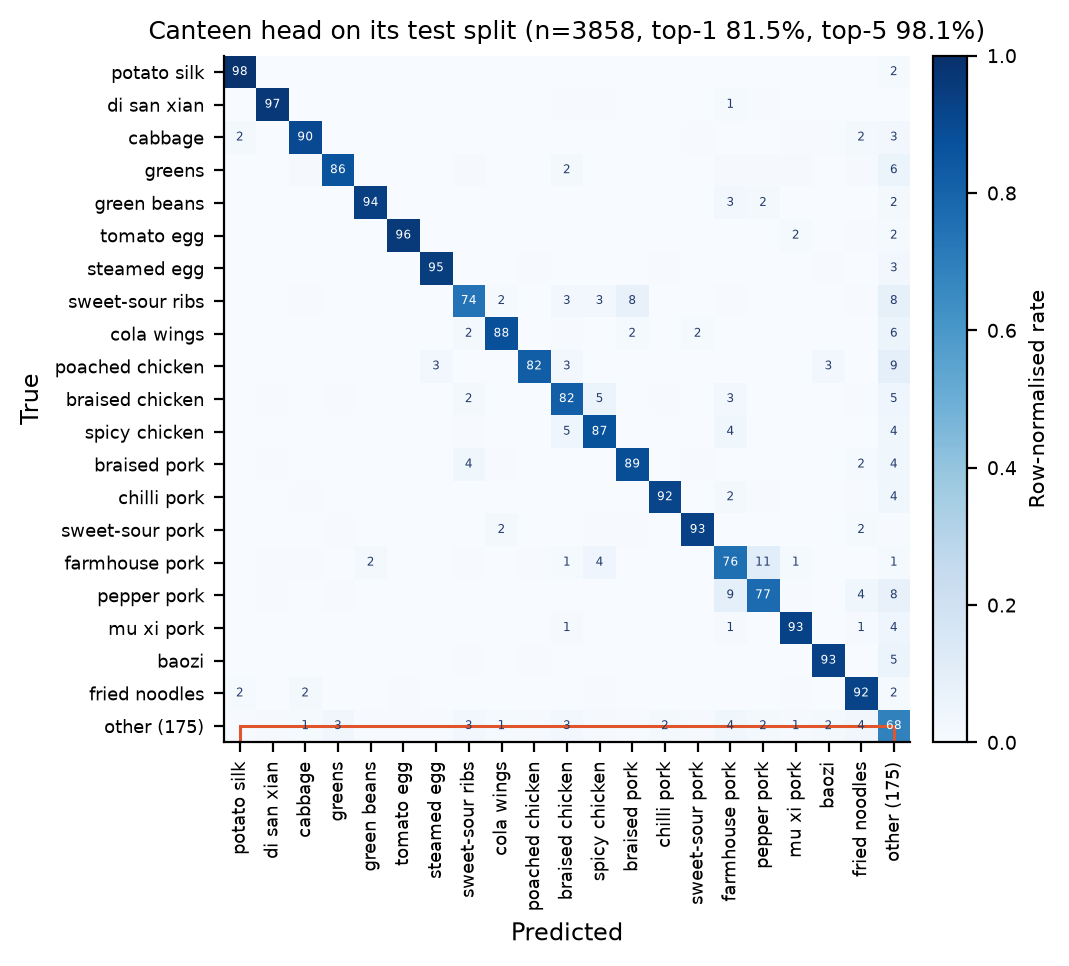
\includegraphics[width=\columnwidth]{cn21_confusion.png}
\caption{Row-normalised confusion matrix of the 21-way canteen head on its test
split, six-view protocol. The red frame marks the catch-all row; its mass leaks
into the generic stir-fries rather than spreading uniformly.}
\label{fig:cnconf}
\end{figure}

\subsection{Open-Set Behaviour}
\label{sec:openset}
Table \ref{tab:gate} and Figure \ref{fig:gate} report acceptance on six sets.
Without the domain probe the gate is already useful: it rejects 85\% of non-food
scenes, 77\% of fifteen unseen Chinese dishes and 82\% of real photographs of
sixteen Western dishes, while keeping \gateInOff\% of the supported test set. The
domain probe then removes a further 7.2 points of unseen Chinese dishes and 9.9
points of non-food scenes, at a cost of \gateInCost{} points of coverage on the
supported set and \gateValCost{} points on validation.

The trade is the one a deployed system wants: a rejected photograph costs the
user one retry, an accepted wrong dish corrupts the energy estimate silently.
The cost is not uniform across the menu, and that is the honest weakness of the
design: on the supported set the probe is confident for most dishes, but it
rejects the ones whose photographs look least like a plated canteen dish, which
is why acceptance is 84\% on the test split and only 31\% on the web images of
baozi (Section \ref{sec:web}).

\begin{table}[t]
\centering
\caption{Acceptance rate (\%) of the deployed gate, with and without the domain
probe, at threshold \gateThr. Higher is better only for the first two rows.}
\label{tab:gate}
\small
\begin{tabular*}{\columnwidth}{@{}lrrr@{}}
\toprule
Evaluation set & w/o probe & deployed & $\Delta$ \\
\midrule
Canteen validation (\cnValN) & \gateValOff & \gateVal & $-$\gateValCost \\
Canteen test, 20 dishes (\cnDishN) & \gateInOff & \gateIn & $-$\gateInCost \\
Fifteen unseen Chinese dishes & \gateOutCnOff & \gateOutCn & $-$\gateOutCnGain \\
Non-Chinese food & \gateOutOodOff & \gateOutOod & $-4.5$ \\
Non-food and clutter & \gateOutOtherOff & \gateOutOther & $-9.9$ \\
Real photographs, 16 dishes & \gateRealOff & \gateReal & $-5.0$ \\
\bottomrule
\end{tabular*}
\end{table}

\begin{figure}[t]
\centering
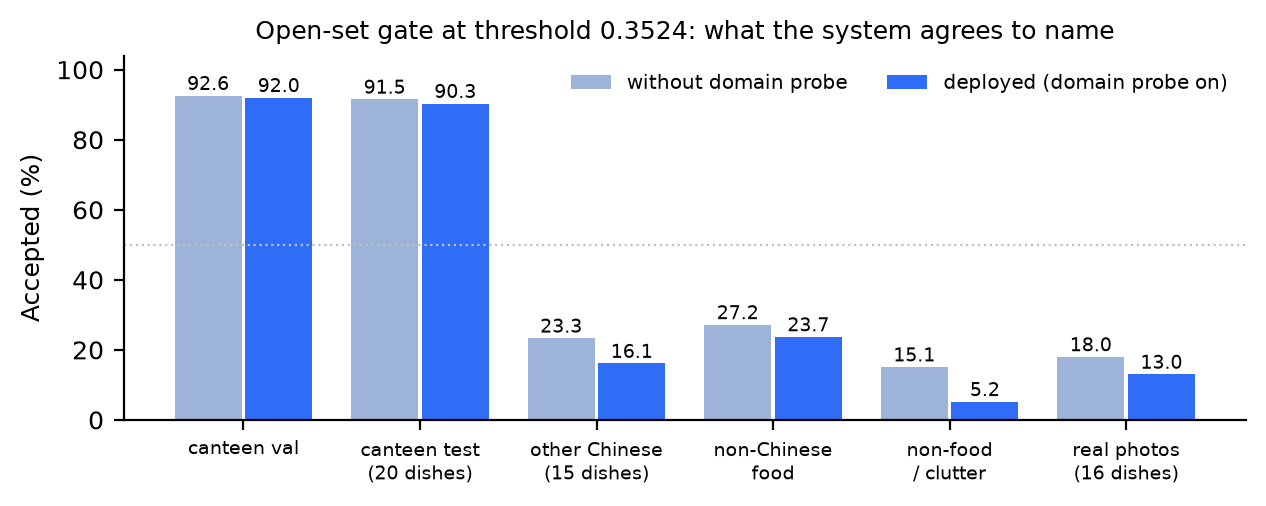
\includegraphics[width=\columnwidth]{cn_gate.png}
\caption{What the system agrees to name, with and without the domain probe. The
supported sets stay above 90\%, the unsupported ones drop to 5--24\%. The
dashed line is 50\% and has no meaning of its own; it only makes the two groups
visually separable.}
\label{fig:gate}
\end{figure}

\subsection{External Evaluation on Web Images}
\label{sec:web}
The \webN{} web images are the only photographs in this paper that no part of
the pipeline has seen. The system is \webTop\% top-1 accurate on them and accepts
\webAccept\%, with \webTopAcc\% top-1 among the accepted ones. Two classes drag
the accuracy down: braised chicken at 75\% and braised pork at 84.6\%, both
confused with sweet-and-sour ribs, which is the same confusion the test split
shows and therefore a property of the classes rather than of the domain.

The acceptance rate is where the web set earns its place. It is \webAccept\%
against \gateIn\% on the test split overall, and the distribution is inverted:
baozi is
accepted 31.6\% of the time and poached chicken 61.5\%, because the domain probe
was fitted on photographs of plated dishes and web images of steamed buns and
poached chicken are shallow-depth-of-field studio shots with no table, no tray
and no context. Measured directly, the web images have a plain border in 0.3\%
of cases against 0.5\% for the test split but a median Laplacian variance of 802
against 505, i.e.\ they are sharper and more isolated than the photographs the
probe was trained on. Removing the domain probe would raise acceptance to 90.2\%
on this set, but it also raises non-food acceptance from 5.2\% to 15.1\%, so we
report the gap rather than tune the threshold on the very set we are reporting.
This is the one place where our external set is not representative: it measures
the menu, not the canteen.

\subsection{Negative Results}
The last four rows of Table \ref{tab:cnmain} are interventions that a reasonable
practitioner would try, and none of them survives.

\textbf{Stronger photometric augmentation} (crop scale 0.45 instead of 0.55,
jitter 0.5 instead of 0.35, hue 0.08, random grayscale with probability 0.1)
moves test accuracy from \cnTest\% to \ablStrongTest\% and top-5 to
\ablStrongTopFive\%, inside the seed spread, while costing three points on
poached chicken and four on mu xi pork. The failure mode is that canteen
variation is not photometric: the same dish is cut differently, garnished
differently and cooked to a different sauce colour, and none of those is a
colour jitter.

\textbf{Class-balanced loss} is the more interesting negative. Inverse-frequency
weights capped at four lift the twenty dishes from 87.4\% to 89.2\% and the macro
average from 86.3 to 88.0, and they fix precisely the weak classes: poached
chicken 82.4 to 94.1, sweet-and-sour ribs 71.0 to 77.9. But the catch-all bucket
loses 9.2 points, from 66.5\% to 57.2\%, and because it holds 36\% of the test
split the total falls to \ablBalTest\%. Pinning the catch-all weight back to one
restores it to 65.3\% and shrinks the dish gain to 0.6 points, netting
\ablBalNoOtherTest\%---a wash. The trade is therefore not in the weights but in
the decision boundary between "one of the twenty" and "something else", and
moving that boundary is exactly what the gate of Section \ref{sec:openset} is
for, with a knob that can be set per deployment instead of baked into the loss.

\textbf{Focal loss} ($\gamma=1$) trades accuracy for calibration: top-5 rises to
\ablFocalTopFive\% and ECE falls to \ablFocalEce, but validation accuracy drops
to \ablFocalVal\% and top-1 is unchanged. Since the displayed top-3 list and the
gate thresholds are both fitted on validation, we keep the cross-entropy model.

\subsection{Complexity, Latency and the Interface}
The deployed model is the ResNet-18 of the Western baseline, so its cost is
unchanged: \paramsFour\,M parameters, \macsFour\,GMACs at $224\times224$, and
\latGpuFour\,ms per forward pass on the GPU. Six views cost six forward passes,
which is still below 25\,ms on this GPU and around 100\,ms on the CPU. The
decision chain that surrounds the forward passes---gate, veto, catch-all test and
threshold comparison---takes \routeCn\,ms per request in the canteen tab against
\routeSingle\,ms in the single-dish tab, both measured on the same machine and
both dominated by the wide-head veto rather than by arithmetic.

The service exposes the three behaviours this paper measures. A supported
photograph returns the top three dishes with posteriors, the energy interval of
Eq.~\ref{eq:interval} and a portion selector; an unsupported one is refused with
the reason (not food, not a Chinese dish, another dish) and, when the refusal
comes from the domain or catch-all test rather than from a weak posterior, the
page offers to retry the same photograph in the single-dish or the 116-class tab.
That suggestion was evaluated offline on 19\,928 requests: when the canteen
tab refuses a real photograph the other tab names the right dish 94\% of the
time, and when it refuses a canteen test image the suggestion is right in only
10 of 300 cases, which is the expected asymmetry---the suggestion is for
photographs that were never canteen food.

\begin{figure}[t]
\centering
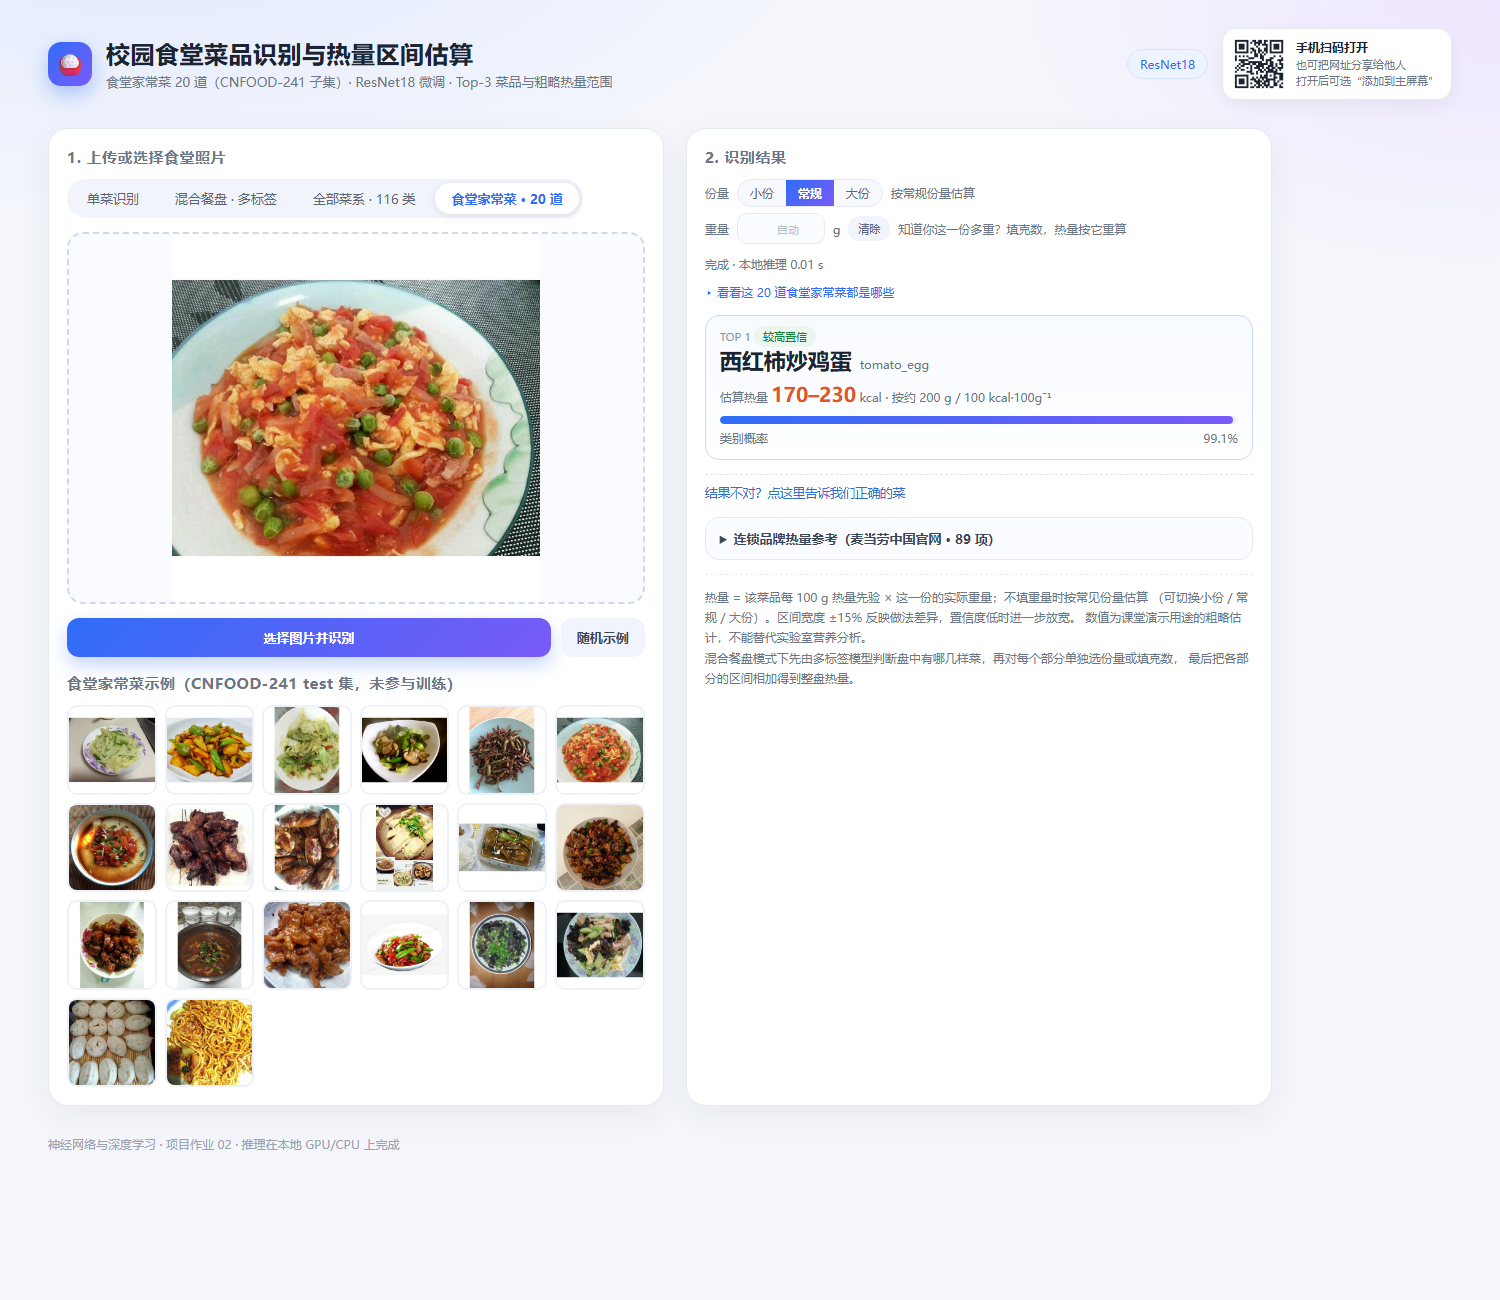
\includegraphics[width=0.95\columnwidth]{demo_cn.png}
\caption{The deployed interface on the canteen tab: top-3 dishes with posteriors,
energy intervals, portion control, and the gate's verdict in the response
payload.}
\label{fig:demo}
\end{figure}

\section{Western Baseline}
\label{sec:baseline}
The project began on a Western menu, and the canteen branch inherits its
methodology: the noise floor, the calibration procedure, the interface and the
complexity measurement were all established here. We report the branch in
compressed form because it answers a different question---how much adaptation
depth and augmentation are worth when the source and target domains are both
curated---and because that answer is the yardstick against which the
pre-training gain of Section \ref{sec:pretrain} should be read.

\subsection{Setup and Main Results}
A twenty-class subset of Food-101 \cite{bossard2014food101} uses the official
split: 600 training, 100 validation and 50 probe images per class from the
official training partition, and the 250 official test images per class as the
in-domain test set (5\,000 images). A proxy canteen domain of 1\,000 images is
synthesized from the probe images with a randomized chain that models a hand-held
phone capture: in-plane rotation up to $\pm7^\circ$, a crop keeping 72--92\% of
each side, a small perspective warp, warm/fluorescent/cool white balance,
brightness in $[0.72,1.25]$, contrast in $[0.78,1.20]$, saturation in
$[0.70,1.30]$, Gaussian and motion blur, vignetting, additive noise,
down-sampling to $320\times320$ and JPEG re-compression at quality 35--65.

Each configuration trains for \epochsFour{} epochs with AdamW, weight decay
$5\times10^{-4}$, head learning rate $10^{-3}$, backbone learning rate
$10^{-4}$, cosine annealing, batch size 64, label smoothing 0.1 and mixed
precision; a run takes \trainTimeFour{} minutes (\epochSecFour{} seconds per
epoch). Table \ref{tab:main} reports the selected checkpoint of every
configuration.

\begin{table*}[t]
\centering
\caption{Western baseline. Accuracy and macro-F1 are percentages on the
5\,000-image official test set and on the 1\,000-image proxy domain; the gap is
test accuracy minus proxy accuracy in points; ECE is computed on the test set;
time is wall-clock training time for \epochsFour{} epochs.}
\label{tab:main}
\begin{tabular}{lccccccrr}
\toprule
ID & Configuration & Test acc. & Test F1 & Proxy acc. & Proxy F1 & Gap & ECE & Time (min) \\
\midrule
E1 & ResNet-18, frozen & \accTestOne & \foneTestOne & \accCanOne & \foneCanOne & \gapOne & \eceTestOne & \trainTimeOne \\
E2 & ResNet-18, frozen + color & \accTestTwo & \foneTestTwo & \accCanTwo & \foneCanTwo & \gapTwo & \eceTestTwo & \trainTimeTwo \\
E3 & ResNet-18, last stage & \accTestThree & \foneTestThree & \accCanThree & \foneCanThree & \gapThree & \eceTestThree & \trainTimeThree \\
E4 & ResNet-18, last stage + color & \accTestFour & \foneTestFour & \accCanFour & \foneCanFour & \gapFour & \eceTestFour & \trainTimeFour \\
E5 & MobileNetV3-S, last stage + color & \accTestFive & \foneTestFive & \accCanFive & \foneCanFive & \gapFive & \eceTestFive & \trainTimeFive \\
E6 & ResNet-18, from scratch (full) & \accTestSix & \foneTestSix & \accCanSix & \foneCanSix & \gapSix & \eceTestSix & \trainTimeSix \\
E7 & E4 + Food-101N (69\,512) & \accTestSeven & \foneTestSeven & \accCanSeven & \foneCanSeven & \gapSeven & \eceTestSeven & \trainTimeSeven \\
E8 & E7 without de-duplication & \accTestEight & \foneTestEight & \accCanEight & \foneCanEight & \gapEight & \eceTestEight & \trainTimeEight \\
\bottomrule
\end{tabular}
\end{table*}

The frozen baseline reaches \accTestOne\% with only 10\,260 trainable parameters,
which already shows how much ImageNet supplies. Unfreezing the last stage raises
accuracy to \accTestFour\% and macro-F1 to \foneTestFour\%, the best of the six
controlled configurations, at zero inference cost. On the proxy domain every
model loses between \gapTwo{} and \gapThree{} points, so photometric and
geometric degradation dominates class confusion within the clean domain.

\subsection{Depth, Colour and Initialisation}
Moving from frozen to last stage is worth \gainFinetuneNoaug{} points without
augmentation (E1 to E3) and \gainFinetuneAug{} points with it (E2 to E4), but
only \gainCanFinetuneNoaug{} and \gainCanFinetuneAug{} points across domains, so
most of the in-domain gain is specific to the clean distribution. Colour jitter
stays inside noise in-domain (\gainAugFrozen{} and \gainAugFinetune) and is the
only factor with a consistently positive cross-domain sign (\gainCanAugFrozen{}
and \gainCanAugFinetune), but the absolute gain is small next to the
\gapFour-point gap it would have to close, which suggests the proxy bottleneck is
geometric rather than photometric.

E6 answers the obvious objection, namely that frozen features already encode
ImageNet. Trained from random initialisation on the same 12\,000 images with every
parameter trainable, the same ResNet-18 reaches \accTestSix\% and \accCanSix\%,
i.e.\ \scratchDrop{} points below E4 in-domain and \scratchDropCan{} across
domains. Twelve thousand images are not enough to learn twenty fine-grained
categories from pixels; the value of the frozen baseline is the prior, not the
10\,260 parameters.

\subsection{External Data and Leakage}
Food-101N \cite{lee2018cleannet} re-releases the same 101 categories from the web
with noisy labels; restricted to our twenty classes it contributes 72\,467
candidates. A candidate is kept only if its released verification label is not
zero and its 64-bit dHash differs by more than a Hamming distance of six from
every validation, test and probe image. The filter removes 2\,495 verified
mislabels and 460 near-duplicates, leaving 69\,512 images, drawn at half weight
against the official images.

E7 moves in-domain accuracy from \accTestFour\% to \accTestSeven\%
(\gainExternal{} points) and proxy accuracy from \accCanFour\% to \accCanSeven\%
(\gainCanExternal{} points), contracting the gap from \gapFour{} to \gapSeven{}
points. The largest cross-domain gain of the study therefore comes from the
photographic diversity of the data rather than from the adaptation policy: web
images vary in exposure, white balance, framing and compression far more than
curated images, which is the effect colour jitter only approximates. E8 repeats
E7 without the near-duplicate filter and gains \leakTest{} points in-domain while
losing 4.6 across domains, so the filter costs nothing and E7 is the configuration
we report.

\subsection{Architecture and Efficiency}
Table \ref{tab:complex} reports complexity and latency. ResNet-18 needs
\paramsFour\,M parameters and \macsFour\,GMACs; MobileNetV3-Small needs
\paramsFive\,M and \macsFive\,GMACs, roughly $30\times$ less arithmetic and
$7\times$ fewer parameters. Latency does not follow the FLOP ratio:
MobileNetV3-Small takes \latGpuFive\,ms against \latGpuFour\,ms on the GPU and
\latCpuFive\,ms against \latCpuFour\,ms on the CPU, so it is \speedCpuFive\%
faster on the CPU but \slowGpuFive\% slower on the GPU, because at batch size one
the cost is dominated by the launch and memory-traffic overhead of many small
depthwise layers. The FLOP saving buys memory and energy rather than wall-clock
time, and the accuracy is \gainMobile{} points lower. This is why the canteen
branch stays on ResNet-18: the compact model buys nothing on the hardware the
service runs on.

\begin{table}[t]
\centering
\caption{Complexity at $224\times224$ input. Params are in millions, MACs in
GMACs (THOP); latency is the mean of 50 single-image forward passes after 10
warm-up iterations.}
\label{tab:complex}
\small
\begin{tabular*}{\columnwidth}{@{}lrrrr@{}}
\toprule
Model & Params & MACs & GPU (ms) & CPU (ms) \\
\midrule
ResNet-18 (E4) & \paramsFour & \macsFour & \latGpuFour & \latCpuFour \\
MobileNetV3-S (E5) & \paramsFive & \macsFive & \latGpuFive & \latCpuFive \\
\bottomrule
\end{tabular*}
\end{table}

\subsection{Cross-Domain Behaviour and Calibration}
Figure \ref{fig:confusion} contrasts the confusion matrices of E4 on the test and
proxy sets. In-domain errors concentrate on the visually similar pairs that
motivated the class selection (dumplings against sushi, pancakes against waffles,
the two salads). On the proxy the diagonal loses mass, the same semantic pairs
survive, and new pairs that share no semantics appear (grilled salmon to caesar
salad, hamburger to french fries). Recall collapses unevenly: french fries keeps
0.84 while hamburger drops to 0.18, consistent with the model losing the evidence
for the class-defining texture and falling back on colour and context.

Both domains stay above the reliability diagonal, so label smoothing plus twelve
epochs leaves the models under-confident rather than over-confident, and the
fine-tuned models are the better calibrated ones (ECE \eceTestFour{} and
\eceCanFour). Post-hoc temperature scaling with one scalar fitted on validation
($T=\tempFour$) lowers test ECE to \eceTestCalFour{} and proxy ECE to
\eceCanCalFour{} without changing a single predicted class. The same procedure,
fitted per branch, is what the canteen head uses.

\begin{figure*}[t]
\centering
\begin{subfigure}{0.44\textwidth}
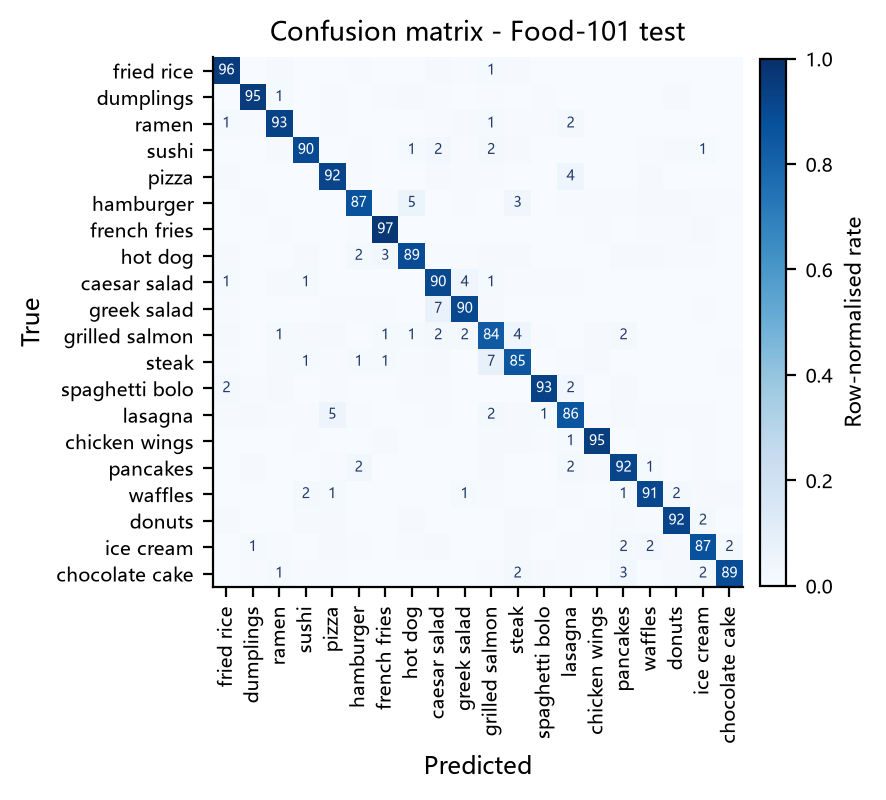
\includegraphics[width=\linewidth]{confusion_test.png}
\caption{In-domain test set}
\end{subfigure}
\hfill
\begin{subfigure}{0.44\textwidth}
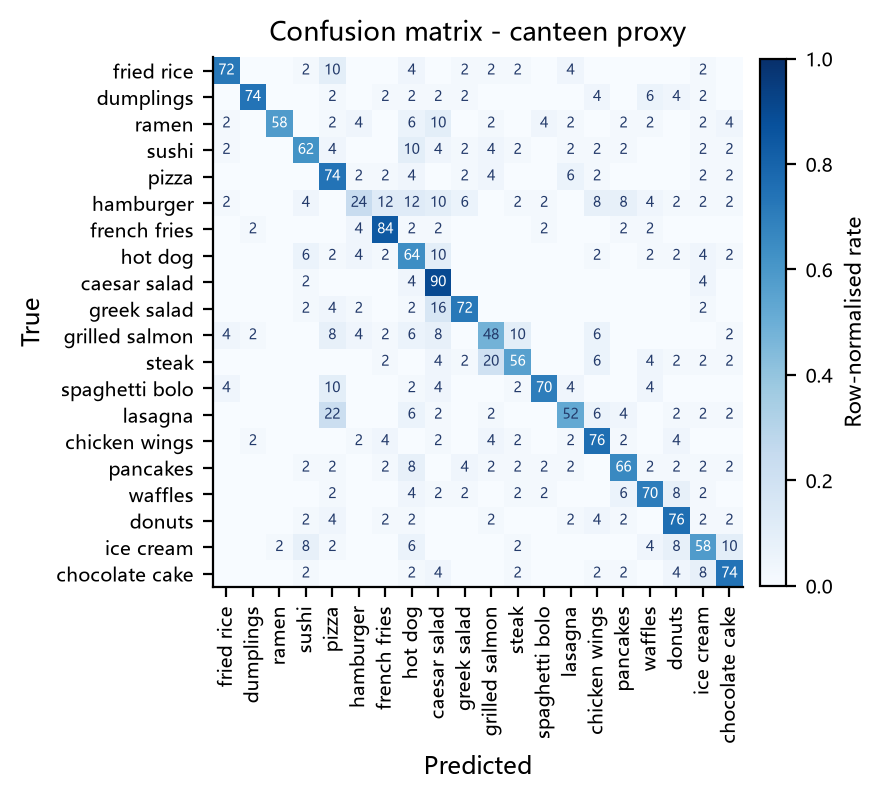
\includegraphics[width=\linewidth]{confusion_canteen.png}
\caption{Proxy canteen domain}
\end{subfigure}
\caption{Row-normalized confusion matrices of the best Western configuration
(E4). Class order follows the class list in the released code.}
\label{fig:confusion}
\end{figure*}

Averaging the softmax over a horizontal flip raises E7 from \accTestSeven\% to
\ttaHflipTestSeven\% in-domain and from \accCanSeven\% to \ttaHflipCanSeven\% on
the proxy; a five-crop average reaches \ttaFiveTestSeven\% and \ttaFiveCanSeven\%,
while multi-scale averaging reaches \ttaScalesTestSeven\% in-domain but falls to
\ttaScalesCanSeven\% on the proxy, because re-rendering at a larger short side
removes part of the evidence the proxy was designed to withhold. Test-time
augmentation is worth about one point here, not the \gapSeven-point gap, which is
why the canteen branch invests in six views rather than in scales: the canteen
shift is compositional, not a loss of resolution.

\subsection{Deployed Interface}
The service is a FastAPI backend that loads the checkpoint once and a single page
that lets the user upload a photograph or pick a bundled sample. The response
contains the top-3 dishes with posteriors, the energy interval of
Eq.~\ref{eq:interval} for each entry, and an uncertainty flag; a portion selector
and a mass field rescale every entry on the client without a new forward pass, so
the user sees how much of the range is recognition uncertainty and how much is
serving size. A second tab handles mixed trays with 40 independent sigmoids
trained on composited plates, and a third exposes the 116-class wide head. Two
learned vetoes sit in front of the classifier, both logistic regressions on the
pooled 512-dimensional feature the classifier already computes: the food veto
rejects 96.9\% of 131 non-food photographs while keeping 95\% of 100 real
canteen dishes, and the packaging veto rejects all 62 audited product cartons at
the price of 0.5\% of dish images. Corrections are collected under every result
as a JPEG plus a CSV row, which is the mechanism the canteen branch inherits.

\section{Discussion and Limitations}
\label{sec:lim}
\textbf{The external set measures the menu, not the canteen.} The \webN{} web
images are the strongest evidence in this paper that the twenty-dish head
generalises, and they are also its weakest link: they are studio-lit photographs
of single dishes, so they share the capture style of the training data and not the
capture style of a tray. The acceptance rate exposes the mismatch (31.6\% on
baozi against 84.4\% overall) precisely because the domain probe was fitted on
plated dishes. A real canteen test set of a few hundred trays remains the
missing experiment, and no amount of web screening substitutes for it.

\textbf{Portions are not measured.} The energy interval covers recipe variability
and, through the confidence term, recognition uncertainty, but the mass comes from
a reference value or from the user. Reported intervals are therefore correct
about the dish and optimistic about the plate.

\textbf{One seed per configuration.} The Western baseline was re-run with a second
seed and moved half a point, which we use as the noise floor. Every canteen
number is a single draw, and the three negative results are negative partly
because their effects are smaller than that floor. The 24-epoch control on the
baseline (E12) shows that the budget is not the binding constraint, and the two
pre-training runs differ by \cnGainPretrain{} points, far above the floor, so the
main claim does not depend on the seed.

\textbf{The gate is a heuristic stack.} A logistic probe, a veto from a wider
head, a catch-all posterior and two auxiliary detectors are combined by
thresholds fitted on validation. Each component is simple and inspectable, but
the composition is not a single calibrated open-set model, and the thresholds do
not transfer to a new canteen without refitting. Reporting coverage alongside
rejection is our attempt to keep this honest; a proper treatment would calibrate
the gate on a held-out tray set, which we do not have.

\textbf{The Western baseline is kept, not discarded.} The twenty Food-101 classes
and the synthetic proxy answer a different question from the one a Chinese
canteen asks, and we report them as the baseline branch rather than as
contributions. Their value here is methodological: the noise floor, the
calibration procedure and the interface were all established there, and the
pre-training gain reported above is only interpretable against that background.

\section{Conclusion}
We presented a canteen dish recognition system for a Chinese campus menu, built
on CNFOOD-241, and measured the three things that decide whether it works.
Pre-training on 241 Chinese dish classes is worth \cnGainPretrain{} points over
the same recipe started from ImageNet weights, more than any adaptation-policy or
augmentation change we could obtain, and it costs nothing at inference. Six-view
test-time fusion adds \cnFuseGain{} points on top, because a tray photograph has
no canonical crop. The 21-way head, with a trained catch-all bucket, reaches
\cnFuseTop\% top-1 and \cnFuseTopFive\% top-5 on \cnTestN{} held-out photographs,
\cnDishAcc\% on the twenty dish rows, and \webTop\% on \webN{} web images that no
part of the pipeline had seen.

The open-set gate is the part we would defend hardest and the part that needs the
most work. It keeps \gateIn\% of supported photographs while rejecting 84\% of
unseen Chinese dishes, 95\% of non-food scenes and 87\% of real photographs of a
Western menu, at a cost of \gateInCost{} points of coverage. That trade is the
right one for a calorie display, where a silent wrong answer is worse than a
retry, but the thresholds are fitted per deployment and the acceptance rate is
uneven across the menu.

Three interventions that a practitioner would try---stronger photometric
augmentation, class-balanced loss and focal loss---do not survive the noise floor,
and their failure is informative: the residual error is intra-class variation and
the boundary of the catch-all class, not optimisation. The next step is therefore
data, not architecture: a few hundred real tray photographs, labelled by the
people eating from them, which is also what the correction link in the interface
is collecting.

\section*{Acknowledgment}
The author thanks the course staff for the assignment specification, the
maintainers of CNFOOD-241 and Food-101, and the authors of ChineseFoodNet, whose
imagery is part of the CNFOOD-241 release.

\bibliographystyle{IEEEtran}
\bibliography{references}

\end{document}
